\documentclass[a5paper,10pt]{report}
\newcommand{\MyTitle}{De tillresta - Silomiterna}
\documentclass[a5paper,10pt]{article}

\usepackage[utf8]{inputenc}
\usepackage[swedish]{babel}
\usepackage[T1]{fontenc}
\usepackage[pdftex]{graphicx}
\usepackage{calc,xparse,geometry}
\usepackage{wrapfig}
\usepackage[pagestyles]{titlesec}

\graphicspath{ {./../Bilder/} }
\newpagestyle{mine}{%
\sethead[\thepage][{\raisebox{\dimexpr\headheight + \topmargin + \voffset + 1in-0.75in\relax}[0pt][0pt]{
\includegraphics[width = .75\textwidth]{horn}}}][]
{}{{\raisebox{\dimexpr\headheight + \topmargin + \voffset + 1in-0.75in\relax}[0pt][0pt]{
\includegraphics[width = .75\textwidth]{horn}}}}{\thepage}
\setfoot{}{}{}
}
\pagestyle{mine}
\author{Gustav Ruthgård}
\title{\MyTitle}
\date{\today}

\usepackage{xkeyval}

\makeatletter
\define@cmdkey{rpg}[char@]{name}[]{}
\define@cmdkey{rpg}[char@]{class}[]{}
\define@cmdkey{rpg}[char@]{kropp}[]{}
\define@cmdkey{rpg}[char@]{reaktion}[]{}
\define@cmdkey{rpg}[char@]{sinne}[]{}
\define@cmdkey{rpg}[char@]{special}[]{}
\define@cmdkey{rpg}[char@]{width}[\linewidth]{}

\define@cmdkey{move}[char@]{rubrik}[]{}
\define@cmdkey{move}[char@]{beskrivning}[]{}
\define@cmdkey{move}[char@]{grundegenskap}[]{}
\define@cmdkey{move}[char@]{lyckat}[]{}
\define@cmdkey{move}[char@]{mitten}[]{}
\define@cmdkey{move}[char@]{misslyckat}[]{}
\define@cmdkey{move}[char@]{val}[]{}
\define@cmdkey{move}[char@]{width}[\linewidth]{}

\define@cmdkey{scenen}[char@]{typ}[]{}
\define@cmdkey{scenen}[char@]{namn}[]{}
\define@cmdkey{scenen}[char@]{rubrik}[]{}
\define@cmdkey{scenen}[char@]{plats}[]{}
\define@cmdkey{scenen}[char@]{birollett}[]{}
\define@cmdkey{scenen}[char@]{birolltva}[]{}
\define@cmdkey{scenen}[char@]{birolltre}[]{}
\define@cmdkey{scenen}[char@]{width}[\linewidth]{}

\newcommand{\statlabel}{\textsc}

\usepackage{calc,xparse}
\newlength\mycardwidth
\setlength\mycardwidth{.75\textwidth}
\NewDocumentCommand \boxme { O{} }{%
  \fbox{%
    \parbox{\linewidth-2\fboxrule-2.5\fboxsep}{\strut #1}%
  }%
}
\NewDocumentCommand \pageme { O{} O{} }{%
  \begin{minipage}{#1\mycardwidth}
    \centering\boxme[#2]
  \end{minipage}%
}
\NewDocumentCommand \cardme { O{.75\textwidth} +m }{%
  \setlength\mycardwidth{#1-2\fboxrule-2\fboxsep}%
  \fbox{%
    \begin{minipage}{\mycardwidth}
      \centering
      #2%
    \end{minipage}%
  }%
}

\newcommand{\setcharacterstats}[1]{%
  \begingroup
  \setkeys{rpg}{name,class,kropp,reaktion,sinne,special,width,#1}%
  \noindent
  \cardme[\textwidth]{%
    \pageme[.69][\statlabel{Namn}: \char@name]%
    \pageme[.31][\statlabel{\char@class}]

    \pageme[.33][\statlabel{Kropp}: \char@kropp]%
    \pageme[.34][\statlabel{Reaktion}: \char@reaktion]%
    \pageme[.33][\statlabel{Sinne}: \char@sinne]
    \raggedright \textit{S�tt ut +2, +1, 0}

    \pageme[][\statlabel{Specialdrag}:]
    \raggedright \textit{\char@special}
  }
}
\newcommand{\displaymove}[1]{%
  \begingroup
  \setkeys{move}{rubrik,beskrivning,grundegenskap,lyckat,mitten,misslyckat,val,width,#1}%
  \noindent
  \cardme[\textwidth]{%
    \pageme[.69][\statlabel{\char@rubrik}]%
    \pageme[.31][\statlabel{Sl�} +\char@grundegenskap]

    \pageme[.99][\char@beskrivning]

    \pageme[.31][\statlabel{10+}]%
    \pageme[.69][\char@lyckat]

    \pageme[.31][\statlabel{7-9}]%
    \pageme[.69][\char@mitten]

    \pageme[.31][\statlabel{2-6}]%
    \pageme[.69][\char@misslyckat]

    \pageme[.99][\char@val]%
  }
}
\newcommand{\satscen}[1]{%
  \begingroup
  \setkeys{scenen}{typ,namn,rubrik,plats,birollett,birolltva,birolltre,width,#1}%
  \noindent
  \cardme[\textwidth]{%
    \pageme[1][\statlabel{\textbf{\char@typ}}]

    \pageme[1][\statlabel{Rubrik:} \char@rubrik]

    \pageme[.31][\statlabel{Huvudroll:} \char@namn]%
    \pageme[.69][\statlabel{Plats:} \char@plats]

    \pageme[1][\statlabel{Plats:} \char@plats]

    \pageme[.33][\statlabel{Biroll: } \char@birollett]%
    \pageme[.34][\statlabel{Biroll: } \char@birolltva]%
    \pageme[.33][\statlabel{Biroll: } \char@birolltre]
  }
}
\newcommand{\rollformular}[1]{%
  \begingroup
  \setkeys{rpg}{name,class,kropp,reaktion,sinne,special,width,#1}%
  \noindent
  \cardme[\textwidth]{%
    \pageme[.69][\statlabel{Namn}: \char@name]%
    \pageme[.31][\statlabel{Koncept}:]
    \pageme[][\statlabel{R�dsla}:]
    \pageme[][\statlabel{Drivkraft}:]

    \pageme[.33][\statlabel{Kropp}: \char@kropp]%
    \pageme[.34][\statlabel{Reaktion}: \char@reaktion]%
    \pageme[.33][\statlabel{Sinne}: \char@sinne]
    \pageme[][\statlabel{Specialdrag}:]
  }
}
\makeatletter

\begin{document}
\maketitle
%\clearpage
%\clearpage
\part{Spelardrag}
Din rollperson kan utf�ra alla dessa drag som en f�ljd av att du agerar p� olika s�tt i en scen. N�r du s�ger vad din rollperson g�r kan SL d� be dig sl� f�r ett av dessa drag.
\section{Attakera}
\textit{N�r du attackerar n�gon som k�mpar tillbaka v�lj hur}

och sl�r \textbf{+Kropp}
\begin{itemize}
  \item[10+] Du lyckas och undviker motst�ndarens attack.
  \item[7-9] Du attackerar motst�ndaren men till ett pris. Spelledaren v�ljer 1:
  \begin{itemize}
    \item Du tr�ffas av ett motanfall.
    \item Du g�r mindre skada.
    \item Du f�rlorar n�got.
    \item Du g�r av med all ammo.
    \item Du uts�tts f�r ett nytt hot.
    \item Du f�r senare problem.
  \end{itemize}
  \item[2-6] SL g�r ett mjukt eller h�rt drag.
\end{itemize}
\clearpage
\section{Undvika}
\textit{N�r du undviker, blockerar eller parerar skada} sl� \textbf{+Kropp}.
\begin{itemize}
  \item[10+] Du klarar dig helt oskadd.
  \item[7-9] Du klarar dig undan det v�rsta av skadan men spelledaren v�ljer om du hamnar i ett d�ligt l�ge, f�rlorar n�got eller om du inte helt undviker skada.
  \item[2-6] Du reagerar f�r l�ngsamt eller g�r en felbed�mning: kanske undviker du inte alls eller s� hamnar du i ett v�rre l�ge �n du b�rjade i. SL g�r ett drag.
\end{itemize}
\section{Tar skada}
\textit{N�r du uts�tts f�r skada} sl� \textbf{+Kropp}. Har du skydd l�gger du till v�rdet till slaget.
\begin{itemize}
  \item[10+] Du biter ihop och kan forts�tta som vanligt.
  \item[7-9] Du st�r fortfarande p� benen men spelledaren v�ljer:
  \begin{itemize}
    \item Skadan f�r dig att hamna ur balans
    \item Du tappar n�got
    \item Du f�r ett \textbf{allvarligt s�r}
  \end{itemize}
  \item[2-6] Skadan �r �verv�ldigande. Du v�ljer om du:
  \begin{itemize}
    \item �r utslagen f�r resten av scenen(SL avg�r om du �ven f�r ett \textbf{allvarligt s�r}).
    \item F�r ett \textbf{kritisk s�r} men �r vid medvetande (har du redan ett kritiskt s�r kan du inte v�lja detta alternativ igen).
    \item D�r.
  \end{itemize}
\end{itemize}
\subsection{Allvarligt s�r}
S�ret beh�ver n�gon typ av v�rd eller tid f�r att l�ka men blir inte v�rre av sig sj�lvt. Alkohol och sm�rtstillande droger kan ta bort avdraget som s�ret ger om s� bara tillf�lligt.
\subsection{Kritiskt s�r}
S�ret kommer inte l�ka av sig sj�lv utan f�rv�rras. Den som �r kritisk s�rad m�ste ha v�rd inom kort f�r att inte d�.
\subsection{Avdrag fr�n s�r}
Om du har icke-stabiliserade allvarliga och/eller kritiska s�r drabbas du av avdrag, enligt nedan.
Om du har
\begin{itemize}
  \item ...minst ett allvarligt s�r; -1 Kropp
  \item ...ett kritiskt s�r; -1 Kropp
  \item ...b�de minst ett allvarlig s�r och ett kritiskt s�r; -2 Kropp
\end{itemize}
Om du dricker alkohol, tar sm�rtstillande, eller bed�var din sm�rta p� liknande s�tt, neutraliserar du avdraget fr�n dina \textbf{allvarliga s�r} under en kortare tidsperiod, vanligen under en scen. Detta g�ller inte kritiska s�r.
\clearpage
\section{�verblicka}
\textit{N�r du �verblickar situationen} sl� \textbf{+Reaktion}. Vid lyckat kan du st�lla fr�gor till spelledaren. N�r du agerar p� spelledarens r�d ta +1 p� ditt slag.
\begin{itemize}
  \item[10+] St�ll 2 fr�gor.
  \item[7-9] St�ll 1 fr�ga.
  \item[2-6] Du f�r st�lla en fr�ga �nd� men du drar till dig o�nskad uppm�rksamhet eller uts�tter dig f�r fara.
\end{itemize}
Fr�gor
\begin{itemize}
  \item Vad �r min b�sta v�g f�rbi hindret?
  \item Vad �r det st�rsta hotet mot mig?
  \item Vad kan jag anv�nda till min f�rdel?
  \item Vad beh�ver jag vara vaksam p�?
  \item Finns det n�got g�mt h�r?
  \item �r det n�got som �r underligt?
\end{itemize}
\section{L�sa av en person}
\textit{N�r du l�ser av en person} sl� \textbf{+Reaktion}
\begin{itemize}
  \item[10+] St�ll 2 fr�gor.
  \item[7-9] St�ll 1 fr�ga.
  \item[2-6] Du f�r st�lla en fr�ga �nd� men du drar till dig o�nskad uppm�rksamhet eller uts�tter dig f�r fara.
\end{itemize}
Medan du talar med personen du l�ser av kan du spendera dina fr�gor 1 f�r 1 f�r att st�lla deras spelare/spelledaren fr�gor:
\begin{itemize}
  \item Ljuger du?
  \item Vad k�nner du just nu?
  \item Vad t�nker du g�ra?
  \item Vad �nskar du att jag g�r?
  \item Hur kan jag f� dig att ... ?
  \item �r det n�got som �r underligt?
\end{itemize}
\section{Unders�ka}
\textit{N�r du unders�ker n�gonting}, sl� \textbf{+Sinne}. Om du lyckas s� finner du alla direkta ledtr�dar och f�r st�lla fr�gor f�r att f� mera information.
\begin{itemize}
  \item[10+] Fr�ga tv� fr�gor
  \item[7-9] Fr�ga en fr�ga, men svaret kostar dig n�got. SL best�mmer vad; du beh�ver n�gon eller n�got f�r att f�rst� svaret, eller det tar dig extra tid att f� reda p� svaret.
  \item[2-6] Du f�r fr�ga en fr�ga �nd�, men du uts�tts f�r ov�ntad fara eller annan kostnad.
\end{itemize}
Fr�gor:
\begin{itemize}
 \item Hur kan jag f� reda p� mer om vad jag unders�ker?
 \item Vad s�ger min magk�nsla om vad jag unders�ker?
 \item �r det n�got konstigt med det jag unders�ker?
\end{itemize}
\section{�vertala}
\textit{N�r du �vertalar en spelledarperson genom f�rhandling, argumentation eller utifr�n en maktposition} sl� \textbf{+Sinne}.
\begin{itemize}
  \item[10+] Hon ger vika.
  \item[7-9] Hon g�r som du vill men (SL v�ljer):
  \begin{itemize}
    \item Hon �r inte n�jd och ber om mer i geng�ld.
    \item �vertalningen skapar problem vid ett senare tillf�lle.
    \item Hon ger med sig men �r os�ker (�vertalningens effekt �r bara tillf�llig).
  \end{itemize}
  \item[2-6] �vertalningsf�rs�ket har oavsiktliga konsekvenser. SL g�r ett drag.
\end{itemize}

\textit{N�r du f�rs�ker �vertala en rollperson} sl� \textbf{+Sinne}.
\begin{itemize}
  \item[10+] Rollpersonen v�ljer sj�lv om hon ger med sig eller inte, du ger dock b�da effekterna nedan.
  \item[7-9] Rollpersonen v�ljer sj�lv om hon ger med sig eller inte, du v�ljer dock en effekt nedan.
  \item[2-6] Rollpersonen �r fri att g�ra som hon vill och har +1 p� n�sta slag mot dig. Ingen av effekterna nedan g�ller.
\end{itemize}
Effekter:
\begin{itemize}
  \item Hon motiveras att g�ra som du vill (hon f�r +1 p� n�sta slag).
  \item Hon drabbas av tvivel om hon inte g�r som du vill (hon f�r -1 V�lm�ende).
\end{itemize}
\section{Agera under hot}
\textit{N�r du g�r n�got riskabelt, �r under tidspress eller f�rs�ker undkomma fara, ber�ttar SL vad hotet �r}, sl� \textbf{+Sinne} f�r att agera trotts hotet.
\begin{itemize}
  \item[10+] Du g�r det.
  \item[7-9] Du g�r det, men tvekar, blir f�rdr�jd, eller m�ste reagera p� en komplikation - SL ger dig ett ov�ntat resultat, ett h�gt pris eller ett sv�rt val.
  \item[2-6] Det blir konsekvenser, du g�r misstag eller s� uts�tts du f�r fara. SL g�r ett mjukt eller h�rt drag.
\end{itemize}
\section{Sj�lvkontroll}
\textit{N�r du anv�nder din sj�lvkontroll f�r att st� emot psykisk p�verkan eller p�frestning som stress, traumatiska upplevelser och �vernaturliga krafter} sl� \textbf{+Sinne}
\begin{itemize}
  \item[10+] Du biter ihop och kan forts�tta op�verkad.
  \item[7-9] Du st�r emot men anstr�ngningen ger dig ett tillst�nd som varar tills du f�tt tillf�lle att �terh�mta dig. V�lj en:
  \begin{itemize}
    \item Du blir arg, ledsen, r�dd eller skuldtyngd. (-1 V�lm�ende).
    \item Du blir h�nf�rd (+1 Relation till det som orsakar tillst�ndet).
    \item Du blir distraherad (-2 i situationer d�r tillst�ndet begr�nsar dig).
    \item Du hems�ks av upplevelsen senare (SL f�r en h�llhake).
  \end{itemize}
  \item[2-6] Du f�rlorar kontrollen och SL v�ljer mellan att du �r maktl�s inf�r hotet, panikslagen utan kontroll �ver dina handlingar eller  m�r d�ligt av traumat (s�nk V�lm�ende enligt traumats styrka).
  \begin{itemize}
    \item Allvarligt trauma (-2 V�lm�ende)
    \item Livsavg�rande trauma (-4 V�lm�ende)
  \end{itemize}
\end{itemize}
\section{V�lm�ende}
V�lm�ende �r ett m�tt p� hur pass balanserat rollpersonens psyke �r. En rollperson �r till en b�rjan kontrollerad men kan sjunka i V�lm�ende n�r hon �r med om traumatiska upplevelser.
\begin{table}[!h]
\begin{tabular}{|c| l l|}
\hline & Kontrollerad & \\
\hline & Olustig & \textbf{Lindrig stress:} \\
& Ofokuserad &  \textit{-1 Sinne} \\
\hline & Skakad &  \textbf{Allvarlig stress:} \\
& Stressad & \textit{-1 Sj�lvkontroll, -2 Sinne} \\
& Neurotisk &  \\
\hline & �ngestdrabbad &  \textbf{Kritisk stress:} \\
 & Irrationell &  \textit{-2 Sj�lvkontroll, -3 Sinne} \\
 & Okontrollerad &  \\
\hline & Nedbruten & Spelledaren g�r ett drag \\
\hline
\end{tabular}
\end{table}
\section{Hj�lpa eller motarbeta}
\textit{N�r du hj�lper eller motarbetar en annan rollperson}, sl� och l�gg till ditt attribut f�r samma drag som den andra rollperson sl�r f�r.
\begin{itemize}
  \item[10+] Ge rollpersonen +2 eller -2 p� slaget.
  \item[7-9] Ge rollpersonen +1 eller -1 p� slaget.
  \item[2-6] N�got g�r fel f�r dig. SL g�r ett drag.
\end{itemize}


\clearpage
\chapter{Bakgrund}
\section{Timelocks}
Tidslås skapas genom att sätta upp enormt kraftfulla Timeflux enheter. Dessa enheter existerar i alla fyra dimensioner och är så kraftfulla att de inte går att förgöra förens deras kraftkällor börjar sina. Tidslåsen gör det näst intill omöjligt att resa tillbaka till den perioden. Ända sättet att manipulera tiden under ett tidslås är att helt enkelt bara ha en fungerande organisation som lever vanliga liv utan tidsresande.
\section{Agentaktiviteter under tidslåsen}
Det första stora tidskriget som pågått i 192 år avslutades 1502 när Leonardo Da Vinci offrade sitt liv för att etablera en enormt kraftull Timefluxenhet. Tidsresor in i tidskrigets slut blev väldigt frekventa och många justeringar genomfördes för att få in så många agenter som möjligt i olika hemliga sälskap. Illuminati, tempelherreorden och många andra slutna sällskap blev grogrunden för dessa agenter. De skapade skrifter om vad deras efterkommande skulle leta efter för tecken och hur de skulle bygga upp organisationen för att hålla människorna i skack.
\subsection{Rebellerna - Människorna}
Efter att Leonardo avslutat tidsresorna fanns inte många upplysta kvar vilket ledde till att enbart några få som avslöjat någon av agenternas riktiga agendor eller avhoppare från dessa känner till vad som egentligen "finns där ute". Förberedelserna inför tidslåsets upphörande blev därför få. Under 1980-talet är de mest tin foil hats. Och liknande nördar som ingen tror på.
\subsection{Cyprox incorperate - Förgörarna}
I det stora kriget föll Cyprox som de stora förlorarna då de förintats och deras sändpunkter i framtiden avslöjats för Ginnies. Några enstaka celler överlevde och enbart en mindre organisation lyckades hålla fast greppet genom tidens tand. Under 1980 talet finns de enbart kvar i nordkorea förklädda till den statens ledare.
\subsection{Ginnies - Avledarna}
Ginnies blev de stora vinnarna dels på grund av deras kamp mot Cyprox från den sändande epok där kriget mellan parterna också pågår. Ginnies slår sig i allians med Rebellerna och deras ledare Leonardo under slutet av 1480-talet och lyckas på så sätt till slut ta över. Efter att låset kommer på plats har deras tidsarkitekter kommit dit och dirigerar hårt vad som skall hända framåt. De sår sina frön utifrån den kunskap de besitter och lyckas väl med att etablera sig. De har fortfarande stor eller mycket stor maktposition under 1980 talet i form av olika celler runt om i världen. Deras största fästen är i Indien och i USA.
\chapter{1986 året för återkomsten}
Scener från denna tid läggs in i det gemensamma bakgrundsskapandet.
\section{Marylain}
I framtiden sätts nya baser upp för tidsresor och probes skickas tillbaka med hundra års mellanrum, sedan 10 år och slutligen hittar man att vissa probes kommer igenom under början på 1986. Den första agenten kommer fram den 7'e februari. En liten ort i södra USA, Marylain kommer att bli dessa trevande försöks viktigaste plats. Då tidslåset fortfarande gör det mycket svårt att komma fram innan det är avstängt gör att enbart en handfull av resande kommer fram. Alla som når fram har olika uppdrag.
\section{Cyprox}
Cyprox är helt fel ute och tror att Ginnies sin vana trogen etablerar sig i Indien. De hamnar där och bygger sin cell i New Deli. Det tar dem ett antal år att hitta Ginnies agenter vilket gör att deras närvaro i USA är okänd under lång tid.
\section{Ginnies 1986}
Ginnies anländer i byn med två arkitekt en man, Tony Diego och en kvinna Ilena Garsia, och en hacker Jonathan Mercy. De två arkitekterna börjar genast genomföra de förändringar som skall leda fram till att tidslåset faller vid rätt tid. Tony tar anställning i skolan och påbörjar där att värva barn för att få bäst spridning på deras uppdrag. Utvalda elever \textit{vaccineras} och får the cricket gene inplaneterad i sig. De kommer att plockas ca 30 år senare för att vervas in som agenter. Ilena börjar istället på IRS kontoret och gifter sig snart för att få barn.
\subsection{Agenda}
Att börja tippa händelserna mot att tidslåset bryts 2018 så som de vet att det kan göra. För att nå dit behöver de se till att många nog från den lilla orten får möjligheten att utveckla en potent gen. Rätt personer skall sedan identifieras och rekryteras som agenter.
\subsection{Hotet}
\begin{itemize}
  \item[Låg] Arkitekterna börjar bygga upp sina epoker. De etablerar generna och planerar för vilka aktiviteter som behöver komma på plats.
  \item[1:a växeln] Mass spridning av generna genomförs. Utvalda klasser i skolan \textit{vaccineras} för att få genen. Epokerna börjar rullas ut.
  \item[2:a växeln] De vaccinerade börjar följas upp för att identifiera vilka det är. Tidiga tecken på vad som händer de påverkade boxas in.
  \item[3:e växeln] De identifierade familjerna infiltreras och barnen vervas som agenter i tidig ålder.
  \item[Overdrive] Blir de påkomna med allt för hårda bevis undanröjs bevismaterial och vitnen utan pardon.
\end{itemize}
\subsection{Roller}
\subsubsection{Tony Diego}
\textbf{Roll: Arkitekt}\\
\textbf{Drifkraft:} Att sätta upp förutsättningar för att tidslåset skall falla 2018. Tar anställning vid skolan och börjar påverka barnen för att de skall genomdriva hans agenda i framtiden. Han blir vän med barnen och blir deras bästa lärare någonsin. Honom kan man lita på och han är inte som de andra vuxna utan tar hand om dem på ett utmärkt sätt. Tony gifter sig med Angela Tombs som har sonen William. Angela har uppfostrat William själv då hans far drog från Marylain innan William föddes.
\subsubsection{Ilena Garsia}
\bild{namn=Personer/Ilena-Garsia,sida=l}
\textbf{Roll: Arkitekt}\\
Drifkraft: Att sätta upp förutsättningar för att tidslåset skall falla 2018. Tar anställning vid sjukhuset och börjar påverka patienter och organisationen för att genomdriva agenda i framtiden.
\subsubsection{Jonathan Mercy}
% \bild{namn=Ginne-agent,sida=l}
\textbf{Roll: Hacker}\\
Drivkraft: Skaffa många barn som möjligt för att sprida en genen via blodet vilket ger bästa potensen. Tar anställning på IRS kontoret och börjar där bygga upp och koda om system för att förbereda för återkomsten.
\subsection{Platser}
\subsubsection{Marylain elementary high}
En traditionell highschool där de flesta av stadens ungdomar går. Skolan är byggd i två våningar med en stor ljusgård i mitten. Klassrummen ligger ut efter fasadens kanter och ljusgården är byggd i grå granit med balkonger runt om på andra våningen. Utanför huvudbyggnaden finns en asfalterad plan med basketplan och två större flyglar. Den ena flygeln inrymmer sjukstugan där \textit{Tony Diego} jobbar som Skolsyster.
\subsubsection{Saint Lucys hospital}
Saint Lucys hospital är ett litet sjukhus som ligger i hjärtat av Marylain. Sjukhuset har hög standard och kombinerar privat vård med den basala som finns för de som inte har råd med sjukförsäkringen. I sina mingröna och mintblå uniformer går personalen runt här. Ordningen är mycket god och patienterna är över lag väldigt nöjda med den vård som bedrivs. Sjukhusets ledning styrs av Ginnies och deras vänner. Här administreras och tas gene-sprutorna fram. Det hela görs som ett forskningsprojekt för ny diabetesmedicin, något som får stora medel varje år från privata givare. Genom att gå igenom bokföringen och kanske även genom att ha koll på hur forskningsområdet kring diabetes bedrivs finns en liten chans att man hittar att något fuffens är på gång.
\paragraph{Malinda Bell}
Receptionist som hjälper besökare till sjukhuset att hitta de patienter de skall besöka. Permanentat hår, bruna plastglasögon på halsrem. 50 årsåldern.
\paragraph{Paul Hampden}
Ung läkare med mörkt hår, är påväg till lunchrast, hjälper till med forskningen på övertid men är inte fullt insatt i läget. Känner väl till de olika faciliterna på sjukhuset.
\subsubsection{Lagerhus 13}
Ett av lagerhusen nere i hamnen har byggts om till kontor och hideout för Ginnie agenterna. Lagerhuset ligger i en del av hamnen som tidigare användes som fiskehamn men nu är övergiven. Denna plats används enbart i nödfall och har ett kassaskåp där hemliga dokument och planer finns lagrade. Dokumenten är skrivna på Silomitriksa och bör vara mycket svåra för spelarna att förstå ifall de skulle komma över dem då det språket börjar talas om 3000 år. Vissa ord kan kännas igen om någon är språkforskare på morderna indiska språk.
\subsubsection{IRS kontoret}
IRS sysslar med skattekontroller på både privatpersoner och företag. Här finns naturligt en massa register över befolkningen, hur de flyttar, vart de jobbar och så vidare. Det här är den perfekta platsen för våra arkitekter att övervaka och även planera och genomdriva sina sociala akrikteturer. På kontoret i Marylain jobbar \textit{Jonathan Mercy} så snart han får chansen att ordna papper osv. Han kommer också att hjälpa andra som kommer resande med att etablera en trovärdig pappersexistens i den här tiden. Kontoret i Marylain är inte så stort, här arbetar ett 20 tal personer och det är ett litet kontor som är utlokaliserat och täcker in en större region än själva Marylain. Lokalen har traditionella kontor och är över lag ganska sunkigt med renovering senast på 60-talet.
\section{Rebeller 1986}
\subsection{Agenda}
I den lilla orten finns ett antal rednecks, en av dem, Ian Parker såg när Tony kom fram genom tidshoppet och är mycket mistänksam, han har också kontaktats av en avhoppare från Ginnie cellen på orten, en annan kille med alkoholproblem som heter Ben Mathews.
\subsection{Hotet}
\begin{itemize}
  \item[Normal] Rednecks do what rednecks does.
  \item[Låg] Då Ian berättar för Ben vad han sett så inser Ben vad som är på gång. Han börjar berätta om de uråldriga sägnerna om tidsresenärerna.
  \item[1:a växeln] Ian och Ben börjar försöka värva andra till sitt cause.
  \item[2:a växeln] Rebellerna har nu fått med ytterligare 3-4 stycken och de börjar sprida rykten om Tony.
  \item[3:e växeln] Rebellerna börjar hota Tony och söker även efter fler tidresenärer. Alla som beter sig konstigt är skyldiga.
  \item[Overdrive] Rebellerna har fått nog och nu skall Tony och de andra dö!
\end{itemize}
\subsection{Roller}
\subsubsection{Ian Parker}
\bild{namn=Personer/Rebel,sida=l}
Ian Parker såg när Tony kom fram genom tidshoppet och är mycket mistänksam, han har också kontaktats av en avhoppare från Ginnie cellen på orten, en annan kille med alkoholproblem som heter Ben Mathews.
\subsubsection{Ben Mathews}
% \bild{namn=Rebel2,sida=r}
Avhoppare från Ginnies cell i Marylain. Alkoholproblem och desperat. Blir kompis med Ian Parker och inser att det är allvar när Ian berättar att han sett Francis tidshoppa in i nutiden.
\subsection{Platser}
\subsubsection{Stanlies bar and grill}
En klassisk amerikansk bar. Drivs av Tony Tomahawk, en indian som är väldigt råbarkad. Han är vän med Ian trotts att Ian kanske inte alltid har det mest högtravande språket när det kommer till Tony. Stället är kanske inte det mest välbesökta av hela byn, men det har en hel rad stammissar som kommer dit både då och då. Stället har ett gömt rum under ett av förrådsrummen där Tony samlat på sig vapen för en hel pluton rednecks. Tonyt ställer upp och delar ut vapen till behövande rednecks om så krävs för att försvara sig mot skumma tillresta.
\subsubsection{Marylain outback camping} \label{camping}
Maryland outback camping park är ett ställe som var tänkt att locka tursiter till träskområdet där de skulle kunna ställa upp sina fina trailers och ha barbeque partyn på kvällarna. Det slog aldrig igenom och är efter år utan underhåll väldigt slitet och sunkigt. Här står några gamla trailers uppställda som inte tar sig iväg från parken då de inte längre går att köra. Ian bor i en av dessa trailers. Dessutom finns här ett 10 tal andra boenden. Att bo här är högst osäkert då ingen riktigt bryr sig om folk som bor här ute. De kvinnor som sökt sig hit i despiration att få tak över huvudet har ofta fått påhälsning av sina ex-män och blivit både slagna och våldtagna.
\subsection{Bakgrundsscener 1986}
\subsubsection{Ginnies}
\satscen{
  typ = Spelledarscen,
  rubrik = När A's fick sitt agentuppdrag av sin faster innan hon försvann.,
  namn = A: ,
  plats = Hemma hos A's fasters coola funkisvilla.,
  birollett = A's Mamma,
  birolltva = A's Pappa,
  birolltre = A's Farbror
}
\satscen{
  typ = Spelledarscen,
  rubrik = När vi gjorde oss redo för skolresan till Frankrike,
  namn = Halynn Shawcross,
  plats = I väntrummet utanför skolsysterns rum,
  birollett = Halynns Mamma Suzy,
  birolltva = Skolsyster,
  birolltre = Halynns bästa kompis Sara Jones!
}
\subsubsection{Rebellerna}
\satscen{
  typ = Spelledarscen,
  rubrik = När farsan sköt Old Tom,
  namn = C:,
  plats = I pappas trailer en regnig höstdag,
  birollett = Old Tom,
  birolltva = Cs pappa Ian Parker,
  birolltre = William Tombs Old Toms son,
}
\clearpage
\chapter{Scenariots startpunkt - 2018 året då tidslåset låses upp}
Arkitekterna har nu förberett allt, det som behövs nu är några tillräckligt mäktiga människor som kan klara av att stänga ned tidslåset. Att göra det kräver en stark gennärvaro och resursfulla personer. Våra arkitekter har sett till att de utvalda är motiverade att komma tillbaka till Marylain för att starta igång med arbetet. De är inte initierade i varför men var och en kommer få ett frö i sin bakgrund som gör att triggern arkitekterna använder sig av görs extra verksam för dem.
\section{The shining order SOT}
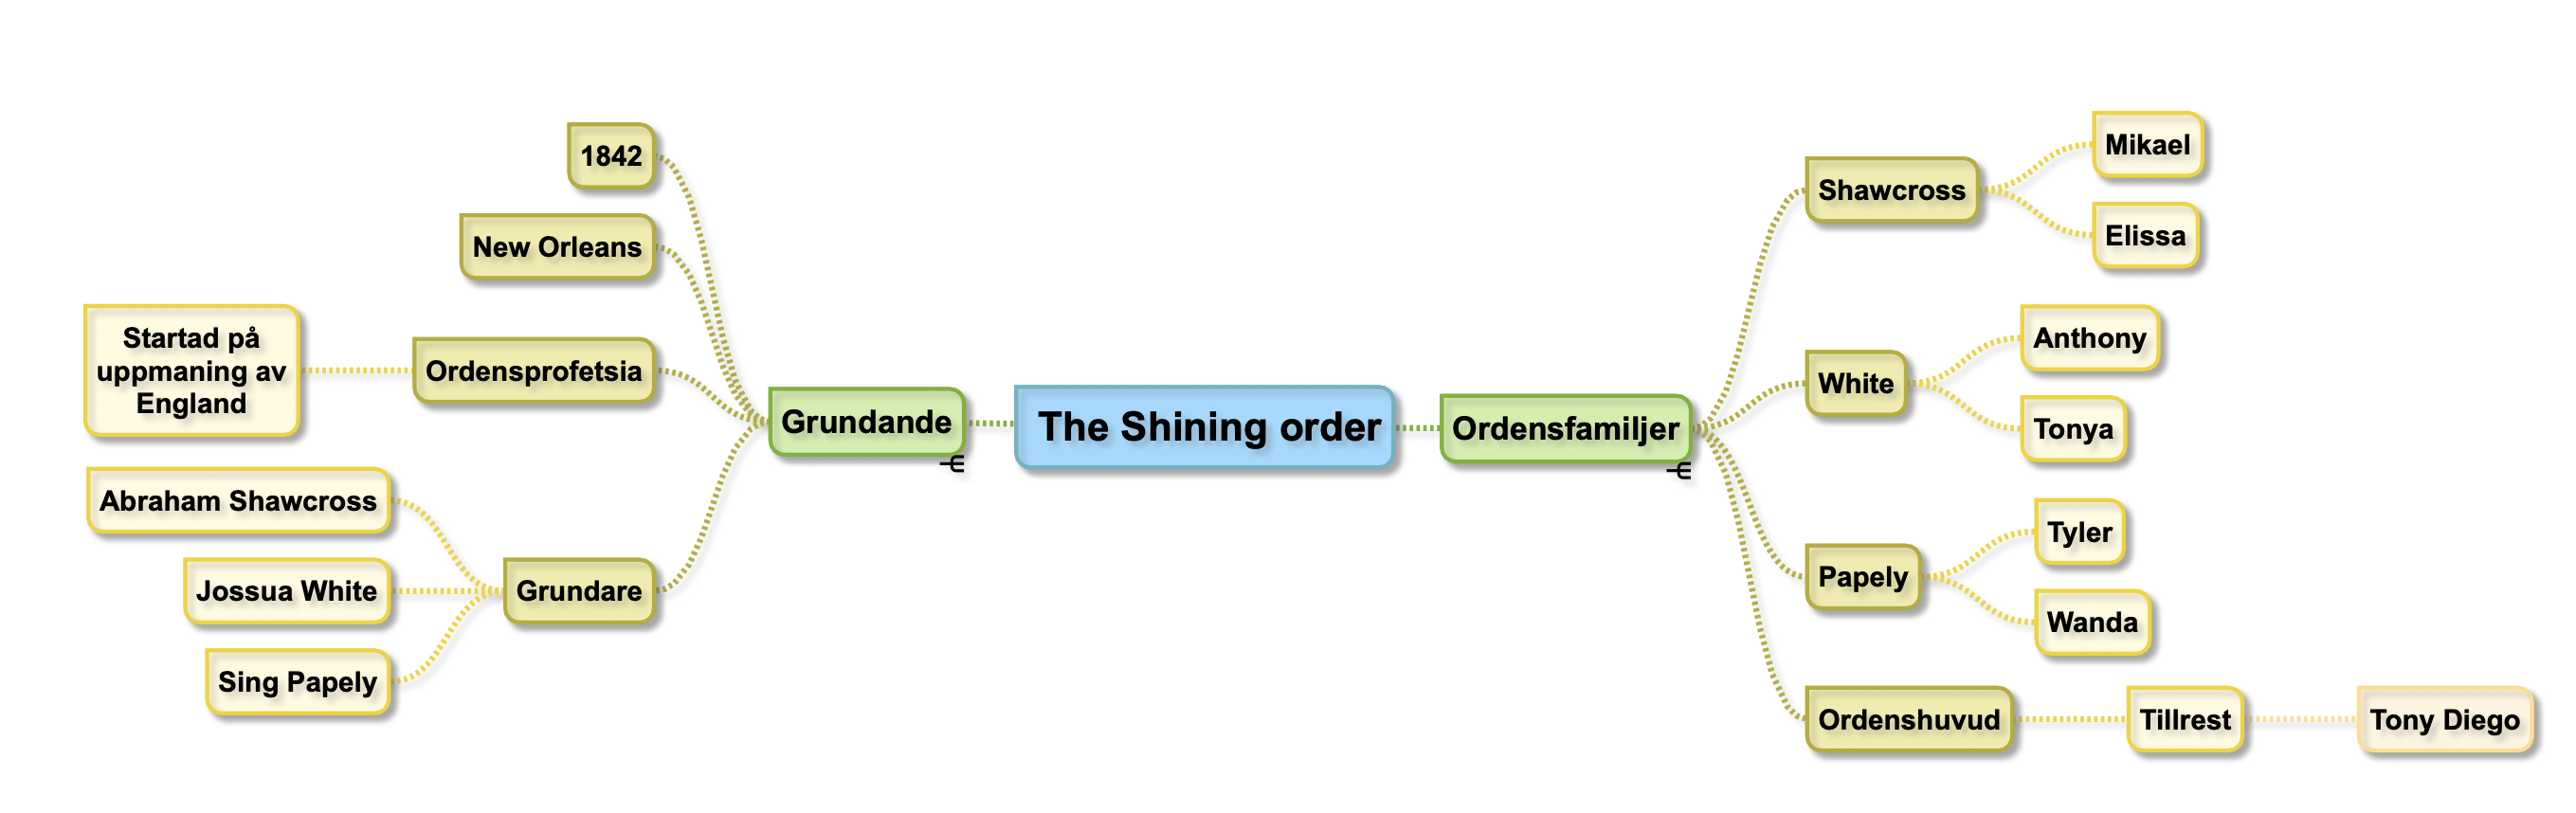
\includegraphics[width=0.9\textwidth]{TheShiningOrder}
The shining order grundades 1842 av två britter och en indier. Abraham Shawcross, Jossua White och Sing Papely. Sing hade under en längre period påverkat de andra två att bli en del av ginnie cellen han startat. Efter en del övertalning och i slutänden utpressning efter att ha sålt några av sina döttrar till de andra två männen som älskarinnor lyckades han övertyga dem att lämna england och etablera sig i New Orleans. Här fick de ett oerhört stort stöd och deras oäkta barn togs in som deras egna. Dessa blev en av de viktigaste fröna till Ginnie cellen i Marylain.
\subsection{Agenda}
SOT har blivit allt mer inflytelserik i Marylain. Sedan Tony klev in som överhuvud i ordern så har de planer som gjorts blivit allt mer framgångsrika. Tony har nyttjat ordern för att driva igenom Ginnies arkitektursplaner.
\subsection{Hotet}
\begin{itemize}
  \item[Låg] Medlemmarna jobbar vidare med sina egna agendor.
  \item[1:a växeln] Rollpersonerna börjar undersöja ordern. Olika underavdelningar kommer nyttjas för att få dem på avvägar eller liknande.
  \item[2:a växeln] Rollpersonerna är påväg att avslöja någon av familjerna som blir desperat. Tony kommer dyka upp för att rädda RP och undanstyra hotet.
  \item[3:e växeln] Någon av familjerna hängs ut och ordern blir väldigt nervös, alla resurser focuseras på att stoppa RP från att störta SOT
  \item[Overdrive] SOT rörelsen hängs ut av RP eller oskadliggörs på något sätt av dem. SOT kommer att gå under jorden. Tony har sett till att alla bevis och en stor skuld kastas mot Italien för att få RP att vilja bege sig dit.
\end{itemize}
\subsection{Roller}
\subsubsection{Shawcross}
En familj med stora tillgångar i Marylain och även i andra delar i USA. Familjen äger stora riskkapitalbolag och har även egna lekbolag inne i Marylain. Familjen är helt oberoende och har därför en väldigt pervers läggning där de torterar unga flickor. Deras dotter har dock flyttat från dem och bor inte längre i Marylain. De har klippt banden till henne fullständigt.
\subsubsection{White}
Ytterligare en mycket framgångsrik familj i Marylain, deras framgångar är mer grundande i politiska sådana, Antony är en mycket skicklig politiker som inte skyr några medel för att gripa mera makt där tillfälle ges. Hans ambitioner är nu än större än när han var borgmästare för Marylain ett antal år tillbaka.
\subsubsection{Papely}
Papely har varit den familj som under alla år har haft hållhakar på de båda andra familjerna och har hållit dme i skack. De har arbetat än mer i de fördålda och verkar på utsidan vara en familj som klarar sig bäst de kan i Marylain. Vid ett antal tillfällen har de dock gått in och tydligt markerat för Shawcross och Whitefamiljerna att det är de som bestämmer i SOT. Tyler Papely är i nuläget sherif i Marylain.
\subsubsection{Tony Diego}
Då Tony anlände till Marylain så visste han att han direkt skulle kontakt Sheriffen Papely för att komma in i Ginnie cellen och kunna börja verkställa sina planer för att förbereda för det arbete som så noga förberetts för att få RP att riva tidslåset.
\section{Front: Ginnies 2018}
\subsection{Agenda}
Arkitekterna har nu gjort det som behövs och nu är pjäserna på plats. Nu gäller det att alla gör sina drag rätt och att allt faller på plats. Tony styr med järnhand och verkar i det fördolda som han är så bra på.
\subsection{Hotet}
\begin{itemize}
  \item[Låg] Pjäserna flyttas och allt går enligt plan, den utlagda väven av manipulation och förändringar skjuter allt i rätt riktning.
  \item[1:a växeln] Rollpersonerna kommer Tony på spåren, han spelar sin roll och är inte rädd att tysta de som står i hans väg. Försiktighet är dock a och o. Han vill inte att huvudsyftet avleds. Att misslyckas nu är inte en möjlighet.
  \item[2:a växeln] Det blir mer och mer kritiskt att händelserna för rollpersonerna mot Italien, de egna kan behöva offras, specialtech och mediciner är medel som kan behöva nyttjas på rollpersonerna för att föra dem i rätt riktning.
  \item[3:e växeln] Rollpersonerna är allierade med rebellerna, inga problem i sig bara de har rätt måltavla, tidslåset måste vara prio ett. Tony försvinner om så krävs.
  \item[Overdrive] Sanningen är påväg att avslöjas, en ny tidsresenär anländer.\footnote{Lägg till en till slp för detta ändamål.} En rad försök att dyka in i tidsepoken trotts att låset ännu inte har fallit görs. Detta kommer synas som elektriska åskbållar som svävar i luften. Det kommer ske på natten ibland och lyser då upp området. Målet för detta är inne i skogen och är samma plats där Tony dök upp. Ben kan peka ut Ian kan peka ut platsen för rollpersonerna men han vet inte om att det har börjat ske igen.
\end{itemize}
\subsection{Roller}
\subsubsection{Tony Diego}
Tony är ledaren för Ginnies i Marylain. Han borde vara i 60 årsåldern men ser ut att vara i 40års åldern snarare. Han har lyckats mycket väl med sina planer för att få RP att vara förberedda för att förstöra tidslåset. Han tar gärna kontakt med dem utifrån att han känner RP från skoltiden. Hans svärson William Tombs är en viktig person i RPs bakgrund som också knyter dem samman med honom. Williams mor Angela har tagit livet av sig för tre år sedan.
\subsubsection{Ilena Garsia}
Ilena Garsia är nu chef för forskningsenheten ADA på \texttt{Saint Lucys hospital} och leder arbetet med forskningen för Cricket gene. Hon har också lyckats få till en ledning på sjukhuset med många ginnie agenter och sympatisörer med hennes forskning.
\subsubsection{Jonathan Mercy}
Jonathan ser mycket bra ut och borde vara i 60 års åldern men ser ut som att han är i 40års åldern. Har varit väldigt framgångsrik, han har lyckats bli chef för IRS kontoret. Dessutom har han lyckats med att få ett 30 tal barn i byn, mycket med hjälp av ett serum från ADA som gör att hans offer helt glömmer bort gårdagen. En handfull av dem har han också som sina egna barn i olika förhållanden han haft. Han är för närvarande singel. Hans huvuduppgift är att bygga pappersspår för de som är tillresta till Mayrilain eller på andra platser runt om i landet men även utomlands.
\section{Front: Rebeller 2018}
\subsection{Agenda}
Rebellerna som först bestod av enbart några rednecks har nu spritt sig in bland gemene man i Marylain. Fronten är inte så enad utan här handlar det om några olika personer som ibland hänger på Stanlies bar and grill. Ben och Ian har blivit allt mer marginaliserade och är inte några personer som tas på allvar i byn. Rebellerna känner sig utsatta och orättvist behandlade och skyller detta på Tony och hans vänner. Rebellerna är misstänksamma mot en rad av de instanser i byn som Ginnies kontrollerar. De vill avslöja dem och åtarta makten till folket.
\subsection{Hotet}
\begin{itemize}
  \item[Låg] Pjäserna flyttas och allt går enligt plan, den utlagda väven av manipulation och förändringar skjuter allt i rätt riktning.
  \item[1:a växeln] Rollpersonerna kommer Tony på spåren, han spelar sin roll och är inte rädd att tysta de som står i hans väg. Försiktighet är dock a och o. Han vill inte att huvudsyftet avleds. Att misslyckas nu är inte en möjlighet.
  \item[2:a växeln] Det blir mer och mer kritiskt att händelserna för rollpersonerna mot Italien, de egna kan behöva offras, specialtech och mediciner är medel som kan behöva nyttjas på rollpersonerna för att föra dem i rätt riktning.
  \item[3:e växeln] Rollpersonerna är allierade med rebellerna, inga problem i sig bara de har rätt måltavla, tidslåset måste vara prio ett. Tony försvinner om så krävs.
  \item[Overdrive] Sanningen är påväg att avslöjas, en ny tidsresenär anländer.\footnote{Lägg till en till slp för detta ändamål.} En rad försök att dyka in i tidsepoken trotts att låset ännu inte har fallit görs. Detta kommer synas som elektriska åskbållar som svävar i luften. Det kommer ske på natten ibland och lyser då upp området. Målet för detta är inne i skogen och är samma plats där Tony dök upp. Ben kan peka ut Ian kan peka ut platsen för rollpersonerna men han vet inte om att det har börjat ske igen.
\end{itemize}
\subsection{Roller}


\section{Marylain geografi}
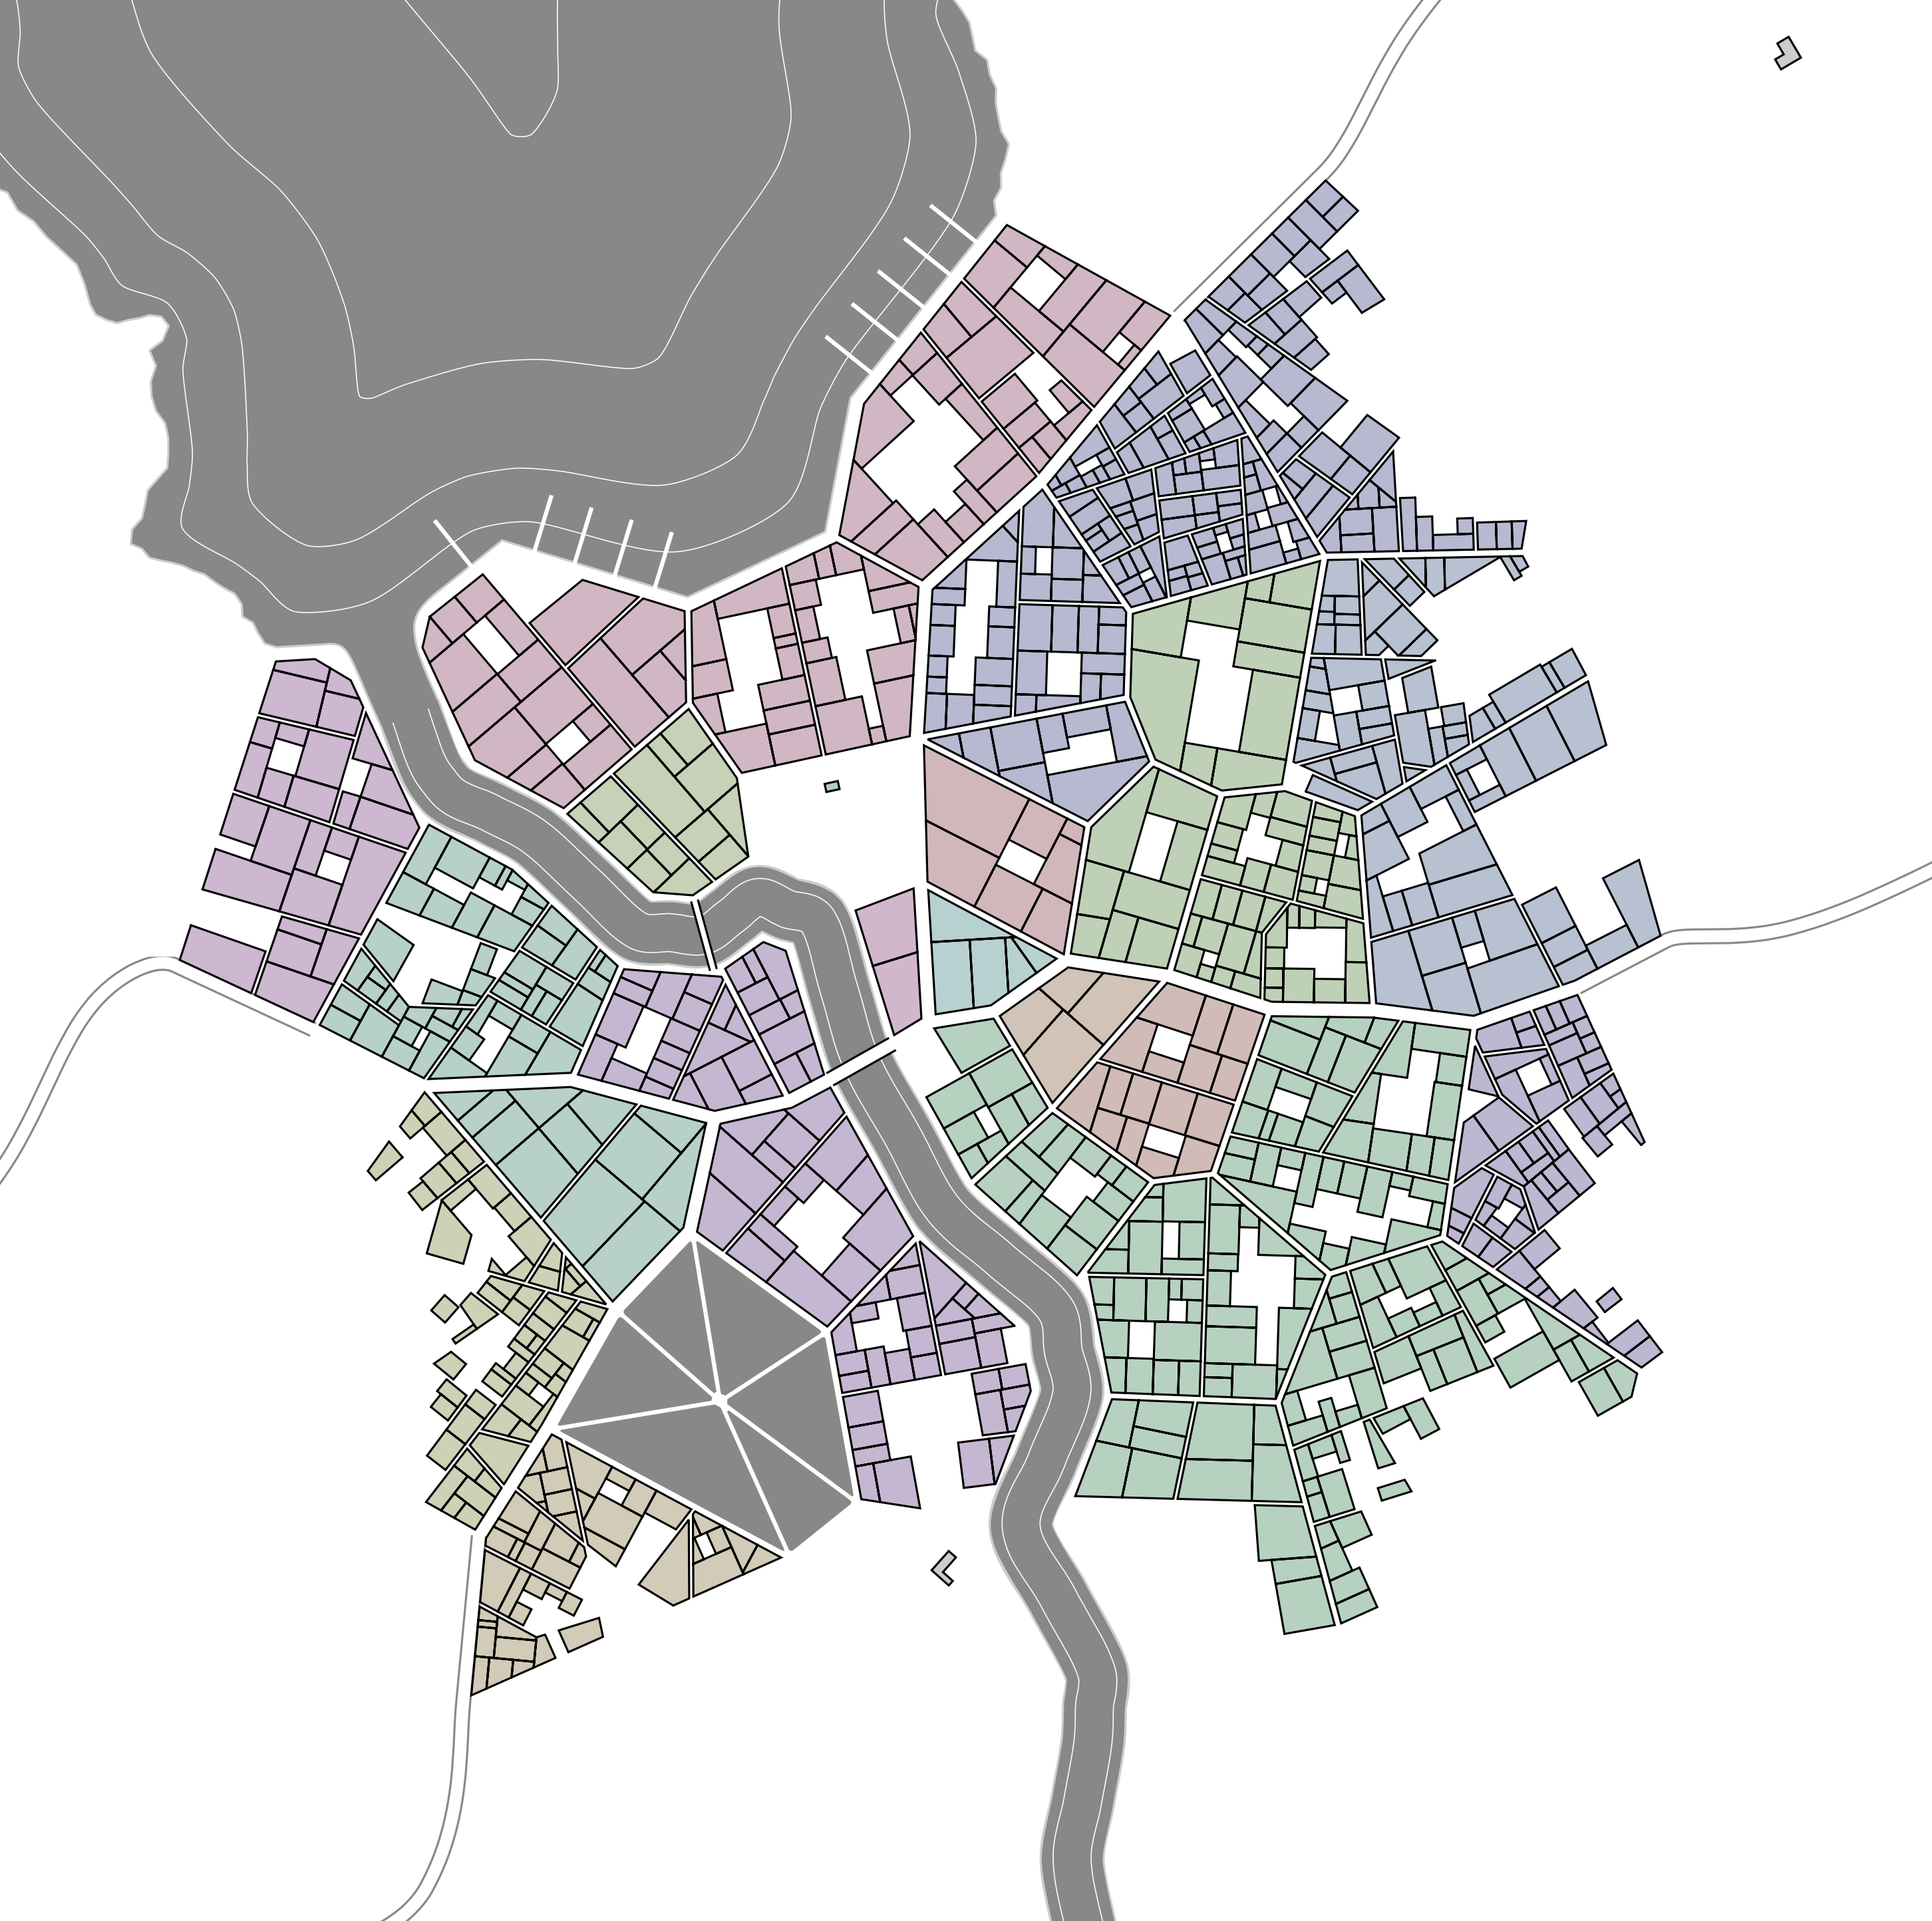
\includegraphics[width=0.9\textwidth]{Platser/Marylain}

Marylain ligger i en sluttning ner mot träskområdet Yellowswamp. Området närmast staden är muddrat och ser mera ut som en sjö. En flod, glass river, rinner sakta ned mot träsket genom staden. Staden består i huvudsak av tre områden.
\subsection{Westside}
Väster om floden ligger ett lite nyare område, byggt på 80 och 90 talet i huvudsak. Här finns en del finare bostadshus och stadens sjukhus Saint Lucys hospital. Här finns även ett IRS kontor.
\subsection{Yellowswamp area}
Den norra delen av staden som gränsar mot träskområdet är benämt efter just detta träsk, Yellowswamp area. Här ligger en hamn som anlades på 1800 talet och ankrade då upp stora flodbåtar som trafikerades från New Orleans. Hamnen nyttjades som just detta fram till 50-talet. Ett antal lagerlokaler finns fortfarande kvar sedan den tiden, de flesta är förfallna men vissa nyttjas fortfarande på detta sätt. Här finns polisstationen.
\subsection{Uptown}
Den sydöstra delen av staden ligger högst belägen och har en fin utsikt ner mot resten av staden. Här finns det äldre finare området med bygnader från början av 1900 talet. Här huserar stadens skola Marylain elementary high och här finns en brokig skara hus i lite olika skick. En av stadens barer finns här, Stanlies Bar and Grill, vilken ligger ner mot floden.
\subsection{Mayrilain outback camping}
Någon kilometer norr om staden öster om träsket ligger Mayrilain outback camping. Utsikten är vacker härifrån ner mot träsket men träd och buskar börjar bli övervuxna och campingen är dåligt skött.
\chapter{Marylain}

\section{Klassfesten}
Alla rollpersoner befinner sig förmodligen i New Orleans dit de flyttat efter att de blivit vuxna. Rollpersonerna kommer alla att delta i en reunionfest för de som bor i New Orleans eller de som har haft möjligheten att resa dit. En av rollpersonerna får vara den som har bjudit in till träffen och får beskriva vart festen hålls, hur den är planerad osv. Alla rollpersoner får beskriva varför de är där och hur de känner inför att återförenas med sina gamla klasskamrater från Marylain high. Då rollersonerna inte har träffats på typ 30 år så är detta ett utmärkt tillfälle att pressentera sig för varndra om vad man nu för tiden gör i livet mm.
\subsection{Klasskamraterna}
\paragraph{Sara Jones}
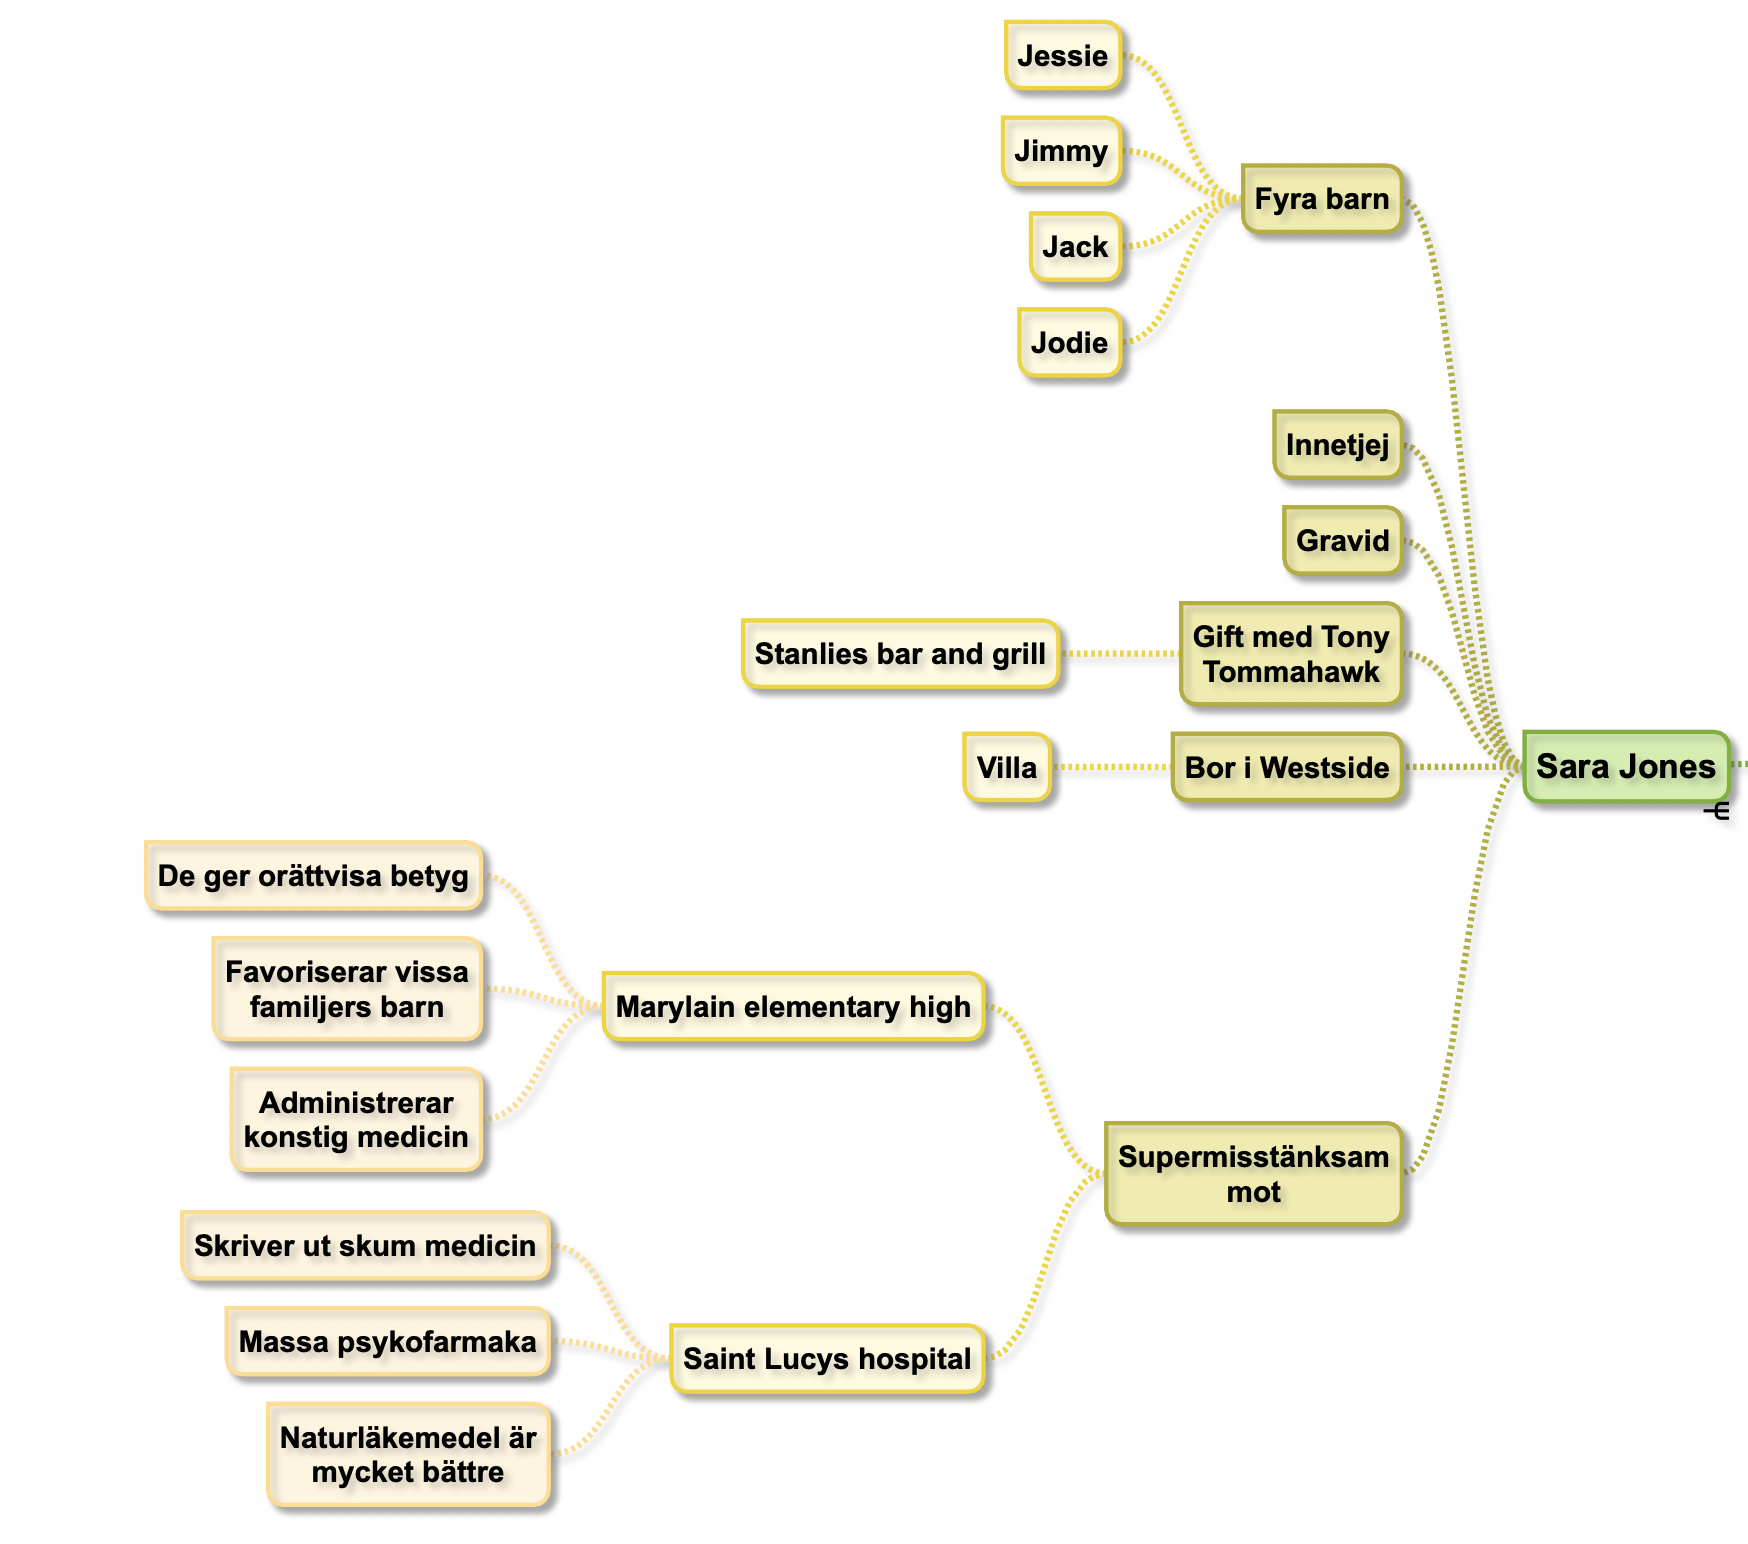
\includegraphics[width=0.9\textwidth]{SaraJonesBubbla}
Sara var klassens innetjej under mellanstadiet. Idag är hon hemmafru och bor fortfarande kvar i Marylain i Westside. Hon har fyra barn, Jessie, Jimmy, Jack och Jodie och är gravid igen så hon dricker inget under festen och poängterar hela tiden hur duktig hennes man är och talar om sina barn och visar gärna bilder av dem. Hon är överviktig och även om hon är garvid så är det bara i andra månden. Hennes man Stanlie Jones driver Stanlies bar and grill. Hon kommer dock att senare på kvällen visa sina misstankar mot både det ena och det andra. Hon kommer rikta misstankar som känns lite ogrundade mot skolan och mot sjukhuset.
\paragraph{Sandra Jefferson - filmen}
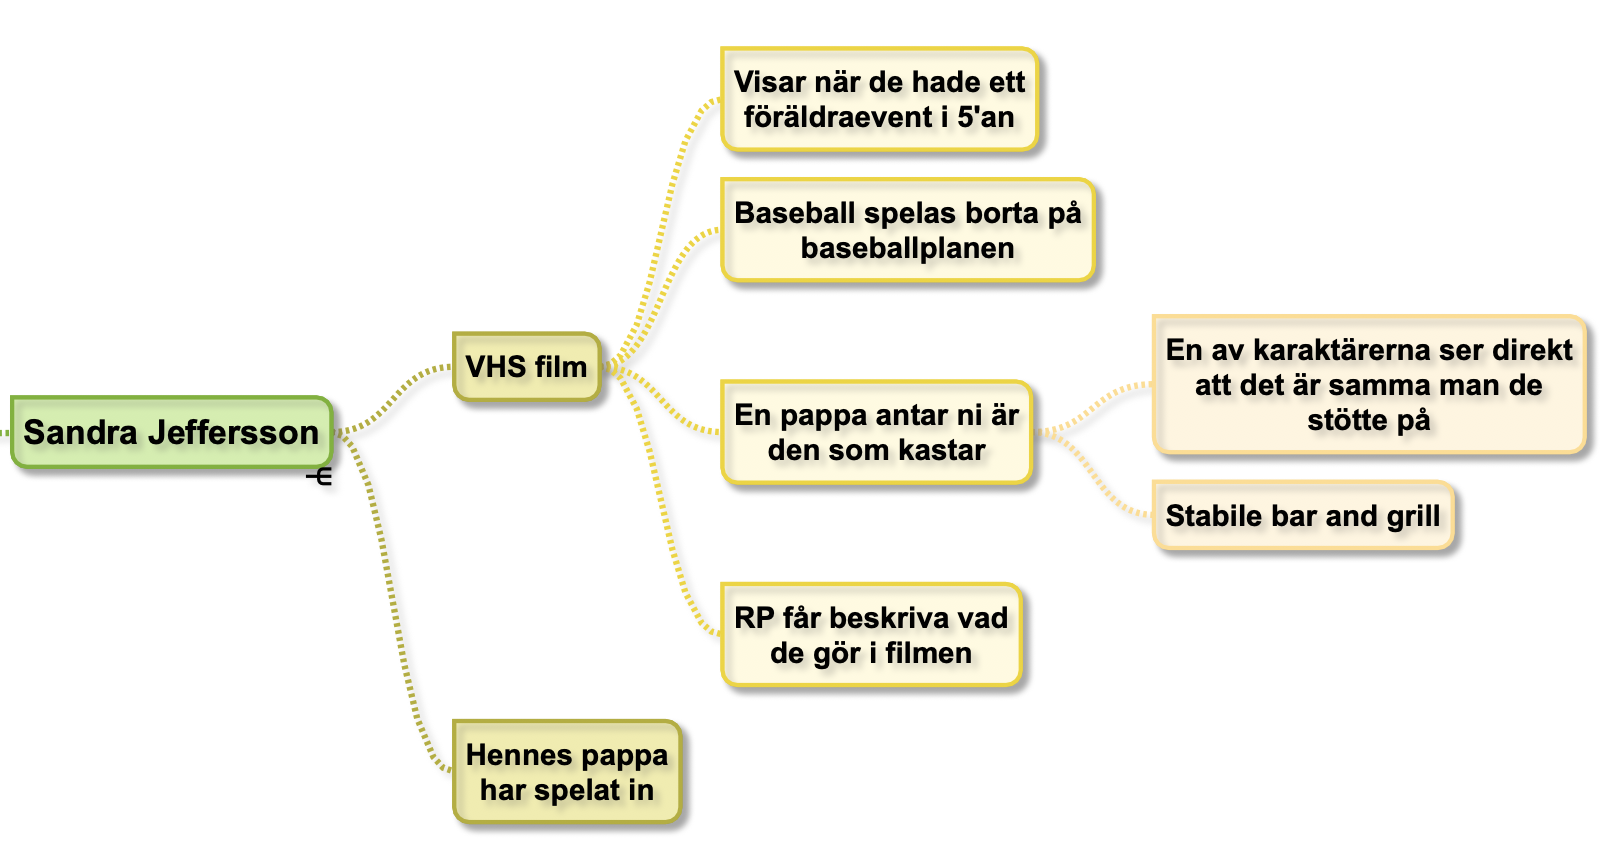
\includegraphics[width=0.9\textwidth]{SandraJefferssonBubbla}
Sandra har plockat med sig en vhs spelare och har med sig en inspelning från klassresan i trean. På filmen spelar klassen baseball och några av föräldrarna är throwers och pitchers. Sandra är glad att få visa filmen som hennes pappa spelat in och den väcker kanske en del minnen från rollpersonerna som får beskriva själva vad de gör i filmen. I slutet av filmen så visas pappan som kastar, det är samma man som någon av rollpersonerna sett på vägen in till Marylain. Mannen har samma ålder som om inte något äldre än den man de såg. Ingen verkar veta vem det var som kastade, kanske kan de hitta vem det är i skolan?
\paragraph{William Tombs - dödssjuk}
Självmordsförsöket av William Tombs. Han har blivit mördad av Ginnies som vet att han kommer att försöka hindra rollpersonerna från att stänga tidslåset. Han är uppvuxen i Marylain camping park. Han har blivit förgiftad vid en vaccinering på sjukhuset och är i väldigt dåligt skick. Han kommer att skicka sms till någon av rollpersonerna om att han är sjuk och att han har blivit inlagd på sjukhuset och därför inte kan komma. Meddelandet kommer från Williams far Tony Diego som är Ginnie agenterna för att inte skapa någon form av misstanke. Tony Diego är Williams styvfar.
\subsection{Namn}
Ella Martin\\
Tanner Billing\\
Marcella Fulmer\\
Richie Skern\\
Cathleen Palmer\\
Alana Deacons\\
Tessa Fisher\\
Odis Evans\\
Rebekah Salford\\
Donn Steven\\
Sophia Fane\\
Tyler Papley
\section{Saint Lucys hospital}
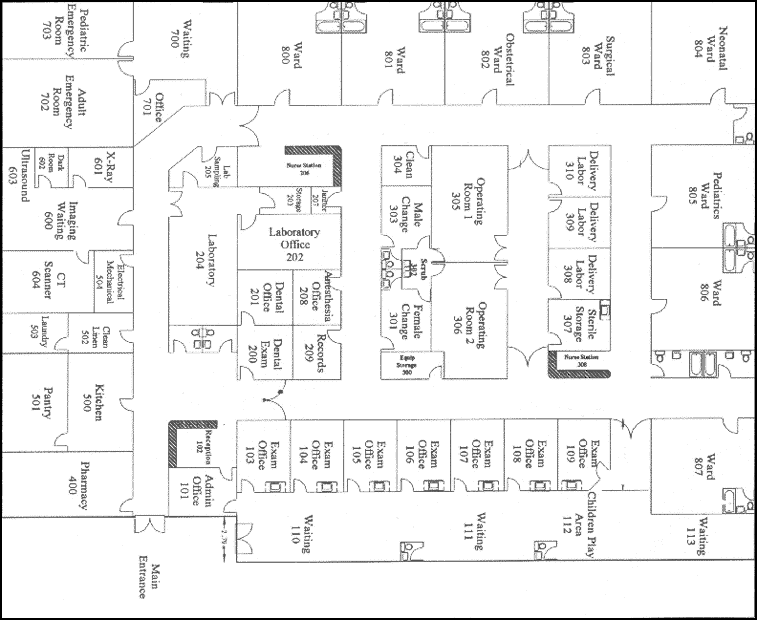
\includegraphics[width=0.9\textwidth]{Platser/Hospital/Hospital-first-floor}

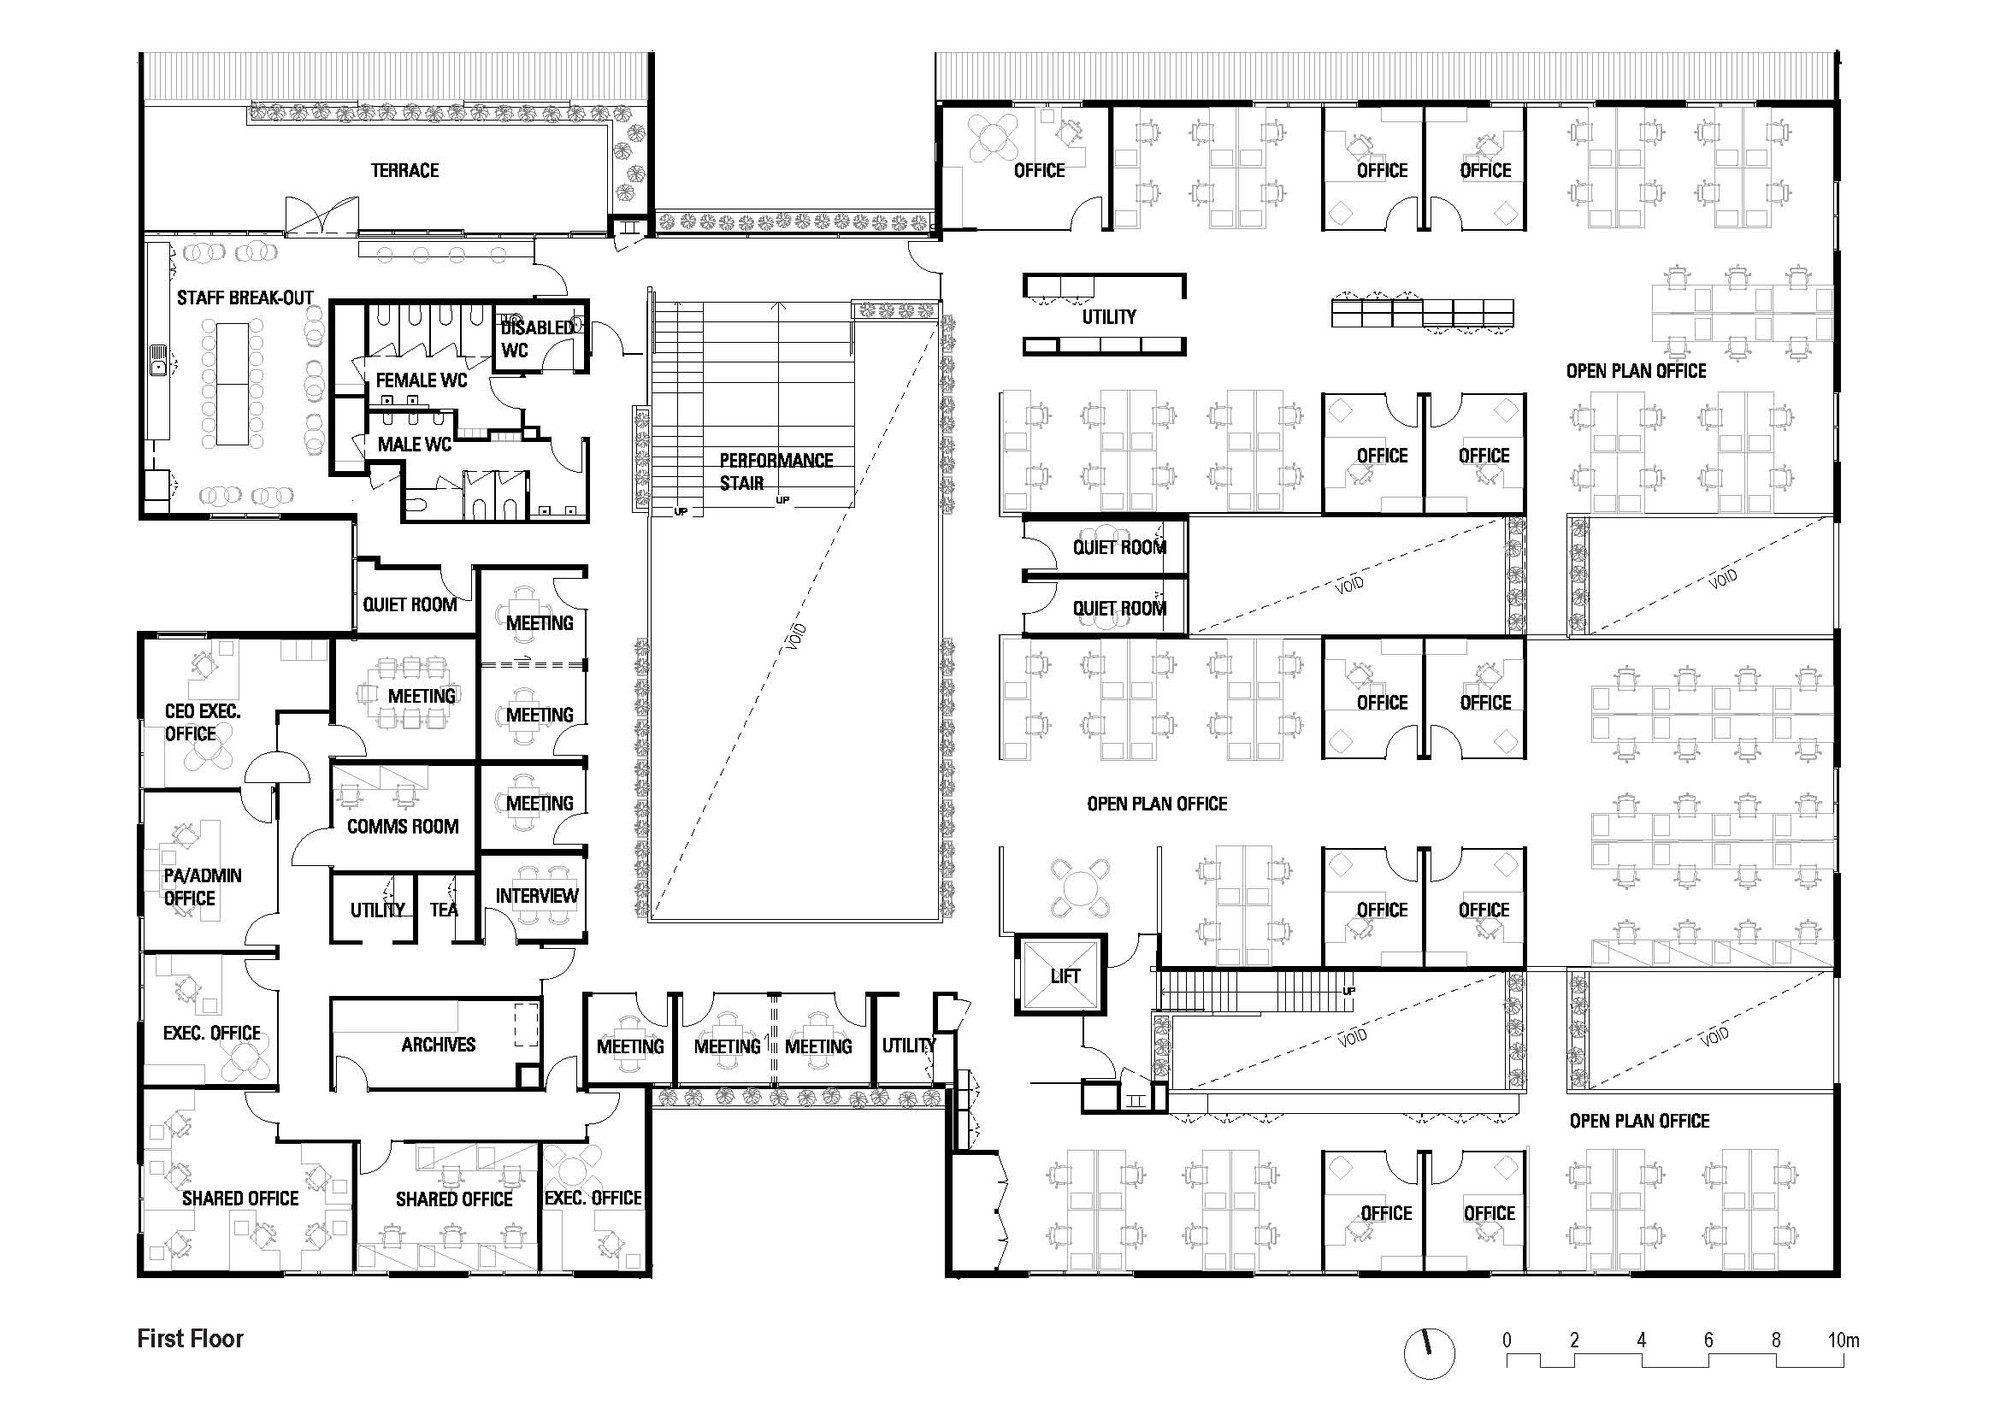
\includegraphics[width=0.9\textwidth]{Platser/Hospital/Second}

För miljöbeskrivning se sjukhuset i Ginnies platslista.\\
% \bild{namn=ada,sida=l}
Sjukhuset har stora anslag om att de vill få forskningsresurer till sitt diabetesteam som jobbar med genombrytande forskning på just diabetesområdet. En doktor Ilena Garsia står som huvudforskare för prjektet på anslaget. Hon ler på bilden och ser inbjudande ut. Här finns en logotyp för ADA American Diabetes Association.
\subsection{William Tombs på sal 5}
William ligger på sal 5 på intensivvårdsavdelningen och är sovande. Han har krafter kvar för att bli väkt om narkosen stängs av. Han har information om att det sista han mins är att han brutit sig in på Lagerhus 13. Där skall det finnas information som pekar på en konspiration i Marylain. Han orkar inte tala så mycket mera innan han till slut somnar in för gott. Om rollpersonerna kollar på Williams tillhörigheter så kommer de att hitta hans hemadress, det är ute i \texttt{Marylain outback camping}. De kan också hitta tändstickor från \texttt{Stanlies bar and grill}. Ingen mobiltelefon finns här.
\subsection{ADA labbet}
Skumheter med forskningen, eget pappersarkiv med olika behandlignar och vad det har lett fram till. Kopplingen tillbaka till skolan där vaccin har givits. Att CG har tillverkats här går att hitta, men vad preparatet faktiskt gör finns inte någon information om.
\section{Marylain police department}
MPD ligger i Yellowswamp area och har en Sheriff \texttt{Tyler Papely} och 3 depudees. Dessutom jobbar det två administrativa medarbetare här. Sheriffen och alla hans depudees är korrumperade till en hög grad av Ginnies. Tony har sett till att han har hållhakar på dem allihopa. Administratörerna är etablerade Ginnie agenter och de har båda affärer med Sheriffen och hans närmste depudee.
\section{God's Empire Gospel Church}
Kyrkan Pastorn \texttt{Franklin Johnson} är Rebell. Här hänger många av de svarta i Mayrilain, men församlingen är en mix och alla är välkomna. Kyrkan är känd för sin duktiga kör och konserter hålls varje söndag. Kyrkan har en ljus och luftig känsla bänkarna är vita och i lackat ljust trä.
\subsection{Pastor Franklin Johnson}
Född och uppvuxen i Marylain med Yellowswamp area. Hans pappa jobbade som dräng på en av gårdarna i närheten och hans mor tog hand om familjen. De har alltid varit väldigt troende.

\section{Stanlies bar and grill}
\subsection{Larry Wade, mannen från filmen}
Här inne finns Larry Wade som kändes igen från filmen Sandra visade. Han kommer inte känna igen rollpersonerna. Om de visar honom filmen så kommer han att bli skakad men försöka bortförklara det med att det måste vara någon annan. Larry jobbar på sjukhuset som sjuksköterska. Han kan om rollpersonerna blir väldigt goda vänner med honom hjälpa dem in på sjukhuset för att undersöka ADA.\footnote{Lägg till Larry som en NPC med beskrivning i Ginnies}
\subsection{Stanlie Jones}
Stanlie kan bekräfta de misstankar som hans fru talat om på klassfesten. Han tror att både Skolan och IRS kontoret är korrupta och har varit under lång tid. Han och flera av hans stammissar har sett märkliga grejjer. Jacob har sett Jonathan Mercy på IRS stå och tittar ut över havet och mäta solupgången med märkliga instrument. Stanlie bar blir extra hårt beskattad, något den blivit sedan han och hans kompisar höjt sina röster och protesterat utanför IRS om att de är korrupta och skumma. Vaccinationsprogrammet på skolan är väldigt märkligt, det är inte det samma som på andra orter.
\section{Marylain elementary high}
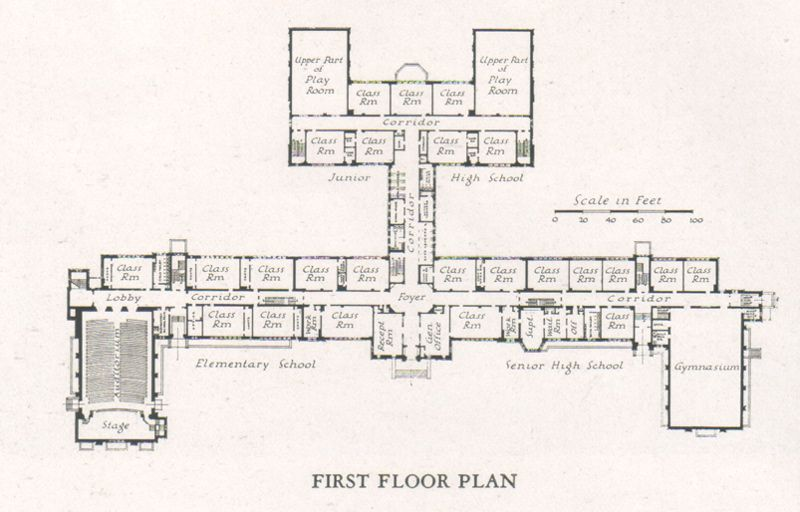
\includegraphics[width=0.9\textwidth]{Platser/Elementary-High/MEH}

Tony Diego\footnote{Ginnies agent} som började som skolsyster är nu rektor. Han har tagit över skolan och diver den nu i egen regi. Studieresultaten är utmärkta och många nya lärare har rest in. Skolan fungerar som mötesplats för Ginnie agenter och hit flyttas de in som har extra stor potential.
\subsection{Lärarrummet}
Här finns en kaffemaskin, en soffa och ett antal bord med stolar. I en av papperskorgarna kan man hitta sönderrivna affischer med reklam för \texttt{Stanlies bar and grill}. På affichen finns en text ditskriven med tusch, \textbf{Jävla Redneck svin}. Texten är skriven av en av de lärare Tony Diego rekryterat som blivit hotad av Ian Parker för att han är en av de som Tony Diego håller bakom ryggen.
\subsection{Rektorns kontor med skolarkivet}
Rektorkontoret består av tre rum, ett sekreteriat där Melissa Borlow jobbar. Hon är otroligt effektiv och skicklig sekreterare och finner stor njutning i att hjälpa Mr Parker. Genom sekreteriatet kommer man in i ett arkivrum och rektorns rum.\\

I rektorns rum finns ett låst kassaskåp som är påkostat, Tony Diego, rektorn, är den ende som har nyckeln och koden till kassaskåpet. Inne i skåpet finns några inlåsta mobiltelefoner, akter på rollpersonerna där deras lämplighet finns inlagda. Här finns även William Tombs akt. Det går också att hitta ett köpebevis på \texttt{Lagerhus 13} från 1984.\\

Det låsta arkivet har skolans bokföring, en rollperson med kunskaper innom bokföring kan här få reda på att stora summor har gått igenom skolan med utbetalningar till Italien. Olika konsultfirmor är mottagare. Pengarna har i första hand kommit ifrån \texttt{Saint Lucy hospital}.\\

\subsection{Skolsysters undersökningsrum}
Undersökningsrummet kommer att skapa flashbacks för rollpersonerna, den scen som finns i deras bakgrund om vaccinet här kommer eventuellt göra att de behöver slå ett \texttt{Självkontrollsslag}. Här inne finns i ett låst skåp som enbart rektorn och sjuksyster Heather Dawnsmith har nyckeln till. Heather är totalt lojal mot Tony och kommer inte lämna ut nyckeln. Skåpet kan dyrkas med ett svårt slag på \texttt{Ta sig in}. I skåpet finns två doser av the cricket gene. Dessa är markerade med CG på flaskan samt ADAs logotyp. Inehållet är genomskinligt. Det finns också ett låst journalskåp där journaler finns. Här är vissa elever förprickade med noteringen CG.
\section{Lagerhus 13}
Lagret är övergivet sedan 1990 talets början och här finns nu några gamla arkiv kvar i kassaskåp av äldre modell. Arkiven innehåller mest stadsplaner, kartor över Marylain och några akter på dess huvudpersoner, den gamla rektorn för skolan, IRS kontorets gamle chef. Med extra svårt att hitta så kan man hitta uppgifter om en plats som måste skyddas för allt i världen. Platsen ligger en liten bit öster om Florens och hit har stora donationer givits, i arkivet finns information om att hundratusentals dollar har givits varje år till en Benjamin Lorenso med adresse i Florens Italien.
\section{IRS}
IRS är mycket svårt att hitta något vid. Allt är digitaliserat och det krävs att rollpersonerna skaffar sig en kontakt som jobbar där för att få ut någon infromation.
\subsection{Jay Fane}
Adopterad Korean, älskar god asiatisk mat, har en hustru han älskar, Simoné. De kan inte få barn. Är svag för hasardspel och har en spelskuld. Är jagad av några av rednecks som bor i \texttt{Marylain outback camping}.
\paragraph{Kan ta reda på:} Att Stanlies Bar and Grill visst betalar extra hög skatt. Något fel har lagts in i systemet. Misstänker att Juliana har en affär med någon på kontoret.
\subsection{Juliana Moland}
Har en affär med Jonathan Mercy och hennes två barn är egentligen hans. Gör vad som helst för att inte bli avslöjad för sin man Dennice Moland.
\paragraph{Kan ta reda på:} Att Jonathan verkar vara väldigt hjälpsam mot nykomna i staden. Han har en otillbörligt hög antal nyregistreringar. Både i Marylain men även en hel del i Italien. Regionen kring Florens verkar vara frekvent förekommande. Den där Amado luktar sprit ibland.
\subsection{Amado Fayneman}
Alkoholproblem, bor i hemlighet i en trailer på campingen. Rädd för hundar.
\paragraph{Kan ta reda på:} Att en del gamla arkiv verkar referera till ett lagerhus 13 i hamnen och en del dokument saknas ur arkiven.
\clearpage
\section{Marylain outback camping}
Campingen har om möjligt förfallit ännu mera med åren. Ett fåtal begagnade vagnar är ditställde under slutet av 90 talet. Annars ser allt ut som förr. Se \ref{camping} för en beskrivning av själva campingen.
\subsection{William Tombs trailer}
\includegraphics[width=0.9\textwidth]{Platser/Marylain-outback-camping/William-Tombs-trailer}

William har under sina vuxna år flyttat hemifrån och valt att bosätta sig där hans riktiga pappa en gång bodde, på campingen. Han har köpt en egen trailer som han dragit dit, den är inte stor men hemtrevlig. William som precis kommit ut som Gay till några av sina närmaste har pimpat den lite för att signalera detta. Trailern är låst men man tar sig enkelt in då låset är dåligt. Trailern har ett rum och är möblerat som säng. Här finns ingen dator och det är stökigt i rummet. I ett par gamla jeans finns ett visitkort till ADA med en tid inskriven på baksidan, tiden är onsdag 13:25. Ingen mobiltelefon finns här.
\clearpage
\subsection{Ian Parkers trailer}

\includegraphics[width=0.9\textwidth]{Platser/Marylain-outback-camping/Ian-Parker-trailer}

Ian parkers trailer med tillbygda skjul är gammalt och slitet. Det finns ganska gott om plats och Ian sitter ofta utanför sitt skjul och dricker Buds. Ian vill gärna rekrytera rollpersonerna till sitt cause och kommer att knyta in i deras bakgrunder om det finns möjlighet till det. Ian för gärna Bens talan om han är där och brer på den sekt som han blev uppfostrad i. Enligt Ian var den till för att hålla varandra om ryggen, ge varandra fördelar och trycka ned de som inte hörde dit. Om rollpersonerna kommer in på det hela så kan han berätta om när Tony hoppade in i verkligheten framför Ians ögon, han vill dock vara säker på att de är på hans sida och kommer att sätta dit Tony innan han berättar.
\clearpage
\subsection{Ben Mathews trailer}
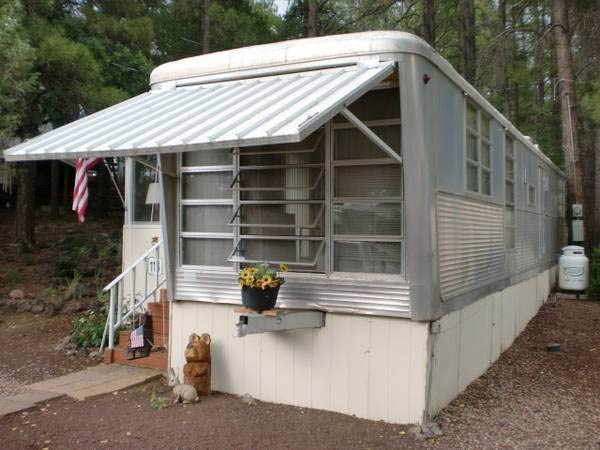
\includegraphics[width=0.9\textwidth]{Platser/Marylain-outback-camping/Ben-Mathews-trailer}

Ben är inte lika social som Ian och säger inte så mycket, han hänger ofta hemma hos Ian och hittas förmodligen där från eftermiddag till efter midnatt. Bens vagn är i gott skick och han fixar ofta med den. Han har också blivit en sam patriot genom åren. Ben kommer tiga om sitt förflutna då han inte gillar att bli sedd som en skummis.
\clearpage
\subsection{Amado Faynemans trailer/shack}
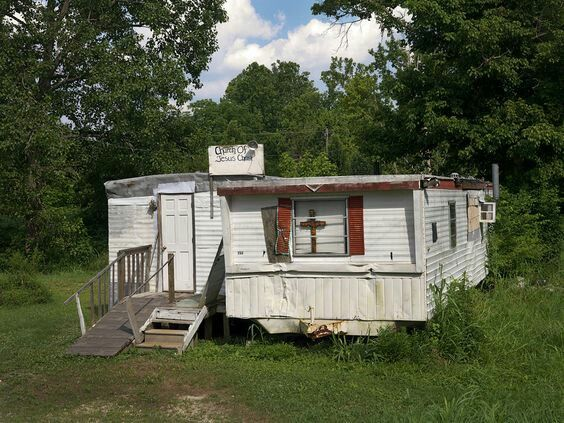
\includegraphics[width=0.9\textwidth]{Platser/Marylain-outback-camping/Amado-trailer}

Trailern var Old Toms trailer en gång i tiden innan han blev mördad. Den har stått övergiven i alla år, William har inte brytt sig om den och det är för många dåliga minnen med den för att han skall vilja komma nära den ens. Nu har Amado Fayneman flyttat in i den då hans alkoholproblem har lett till att han inte längre kan bo kvar i sin lägenhet.
\chapter{Akt 2 - Italien}
Florens
Vinci
Tidskapslarna
Långt inne i en grotta under marken.
Mötet med Leonardo
Tidsvarelser som kretsar runt och skadar Leonardo.
Tidslåset
\clearpage
\section{Gamla noteringar}

Agentscen där en agent rekryterar dem?

Timeflux maskinen
  Tungt bevakad
  Utan avstängningsfunktion

Turn off in all dimensions?
  Sight of the aliens?


\end{document}
